\subsection{Schwerpunktverteilung mit Gleitkommazahlen}
\begin{table}[h!]
    \hspace{-0.75cm}
    \begin{tabular}{ | l | c | c | c | c |}
        \hline
        Konfiguration & Beste & Unter 44 kB & Unter 28 kB & Unter 14 kB \\\hline
        Ensemble-Methode & Boosting & Random Forest & Random Forest & Bagging  \\\hline
        Maximalhöhe & 20 & 12 & 10 & 7 \\\hline
        Waldgröße & 10 & 7 & 4 & 3 \\\hline
        Blattgröße (min\_samples\_leaf) & 8 & 1 & 2 & 8 \\\hline
        Programmgröße in Bytes & 83304 & 43668 & 20188 & 6656 \\\hline
        Genauigkeit Testmenge von Klisch & 94,8\% & 89,6\% & 89,6\% & 87,5\% \\\hline
        Genauigkeit Gestentestmenge & 97,0\% & 96,5\% & 95,6\% & 94,1\% \\\hline
        Genauigkeit Nullgestentestmenge & 92,2\% & 92,4\% & 88,8\% & 89,9\% \\\hline
    \end{tabular}
    \caption{Die besten Konfigurationen der Schwerpunktverteilung mit Gleitkommazahlen.}
    \label{tab:schwerpunktverteilung_float}
\end{table}
\begin{figure}[h!]
    \centering
    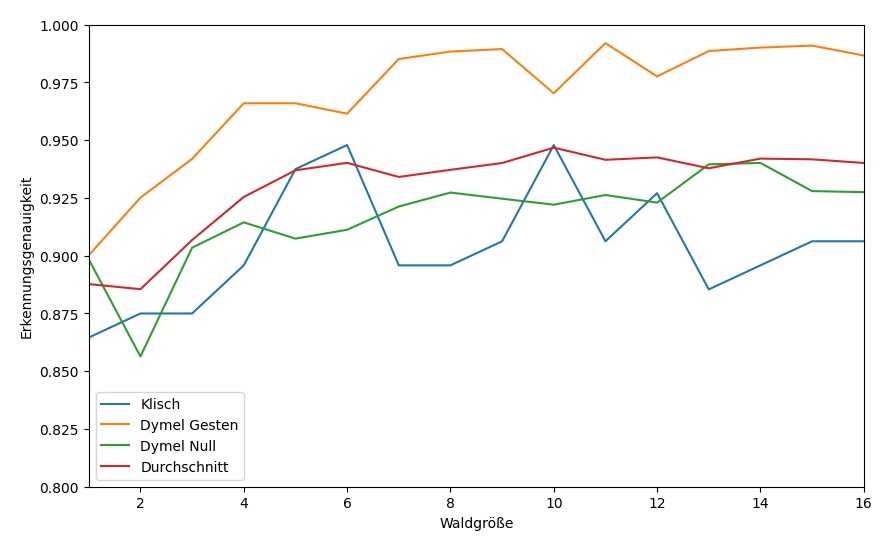
\includegraphics[width=\linewidth]{images/cocd_float_acc_per_size.png}
    \caption{Die besten Konfigurationen pro Waldgröße der Schwerpunktverteilung mit Gleitkommazahlen.}
    \label{fig:cocd_float_per_forest_size}
\end{figure}
Die Feature-Menge Schwerpunktverteilung mit Gleitkommazahlen folgt der Definition aus Kapitel \ref{sec:schwerpunktverteilung} und beinhaltet insgesamt zehn Einträge. Jeweils zwei Einträge bilden die X und Y
Koordinate des Schwerpunktes. Damit spiegeln zehn Einträge insgesamt fünf Zeitfenster wieder.
\newline
\newline
Aus der Tabelle \ref{tab:schwerpunktverteilung_float} sind die besten Konfigurationen jeder Kategorie zu entnehmen. Die beste Konfiguration wurde mit der Ensemble-Methode Boosting gefunden.
Mit einer Klassifizierungsgenauigkeit von 94,8\% auf der Testmenge von Klisch ist dieser Ansatz nur 4,2\% schlechter als das neuronale Netz von Giese \cite{gieseThesis}. Es ist anzumerken, dass mit einer
kleineren Trainingsmenge ohne die Gestentrainingsmenge und Nullgestentrainingsmenge eine Lösung gefunden wurde, die 97,9\% erzielte und damit nur 1,1\% schlechter ist.
Außerdem werden 97\% der Gestentestmenge und 92,2\% der Nullgestentestmenge korrekt klassifiziert.
\newline
\newline
Im Vergleich zu der Helligkeitsverteilung und Motion History ist die Klassifizierungsgenauigkeit dieses Ansatzes signifikant besser, sogar wenn nur 6656 Byte Programmspeicher verwendet werden.
Wird die Kategorie \textit{Beste} mit der Kategorie \textit{Unter 14 kB} verglichen, nimmt die Gesamtklassifizierungsgenauigkeit nur um 4,17\% ab. Dabei wird die Programmgröße um 92\% reduziert.
Dies verspricht, dass mit zunehmender Waldgröße die Klassifizierungsgenauigkeit steigt. Abbildung \ref{fig:cocd_float_per_forest_size} zeigt, dass dies zwar der Fall ist, aber schon ab einer Waldgröße von 6
Bäumen verzeichnet die durchschnittliche Klassifizierungsgenauigkeit keinen signifikanten Zuwachs mehr. Dementsprechend ist der Unterschied der Gesamtklassifizierungsgenauigkeit der Kategorie \textit{Beste}
und der Kategorie \textit{Unter 44 kB} mit 1,8\% nicht groß. Damit eignet sich diese Feature-Menge gut für kleine eingebette Systeme, da nur wenige Bäume benötigt werden.